
\section{Roda Omnidirecional}

A roda omnidirecional aparece em vários modelos na literatura, tais como no design de J. Graboweicki em 1919
\cite{patent_US1305535A} e o de Josef Blumrich em 1972 \cite{patent_US3789947A}. A roda consiste de rolos
perpendiculares à  sua direção de giro, cuja presença tem como efeito conferir à roda a capacidade de se locomover em
qualquer direção no seu plano. Essa capacidade é o que confere aos robôs aqui discutidos suas características
holonômicas, uma vez que as restrições de movimento a que eles estão sujeitos está normalmente atrelada à construção dasrodas \cite{TAKAHASHI}.

\begin{figure}[h]
	\centering
	\caption{Modelo de uma Roda Omnidirecional}
	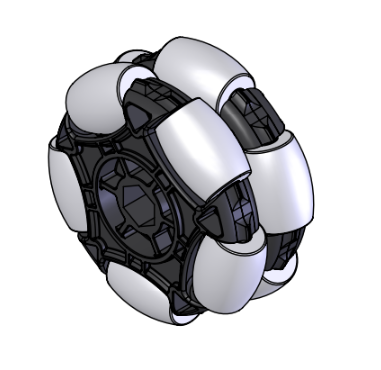
\includegraphics[width=0.5\textwidth]{figures/omniwheel}
    \caption*{FONTE: https://www.vexrobotics.com/omni-wheels.html}
\end{figure}

A relação entre velocidade linear e angular da roda é dada por:

\[V_{w1} = \omega_{w1}\cdot r \] 

em que $V_{w}$ é velocidade linear da roda, $r$ o raio da roda, $\omega_{w} $ e é a velocidade angular da roda.

Uma variação da roda omnidirecional é a roda mecanum, criada por Bengt Ilon \cite{patent_US3876255A} - 
a diferença fundamental entre elas é a construção dos rolos ligados à estrutura central  -
os quais, no caso da roda mecanum, são posicionados a 45°.

\subsection{Obtenção da roda omnidirecional}

Inicialmente foram compradas roda prontas, fabricas fora do território nacional, por meio de importação.
Mas o mesmo modelo pode ser encontrado sendo vendido no Brasil.
O modelo adquirido inicialmente possui diametro de 58mm, largura de 26mm e possui um acoplamento para eixo de 4mm de diametro.
Essas dimensões foram adquadas nos primeiros testes de contrução do robô enquanto se estava usando motores DC,
mas quando o projeto passou a usar motores de passo Nema 17, as rodas não eram mais compatíveis com o eixo e as dimensões dos motores.
(A mudança de tipos de motores será discutida na seção sobre motores).

\begin{figure}[h]
	\centering
	\caption{Roda omnidirecional usada inicialmente}
	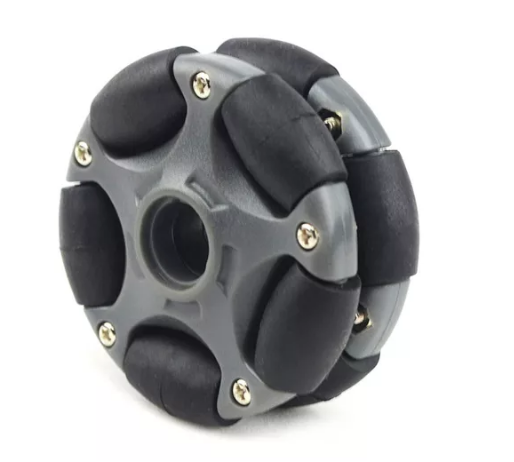
\includegraphics[width=0.5\textwidth]{figures/roda_china.png}
    \caption*{FONTE: https://rapidroboticsaustralia.com/products/58mm-nylon-omni-directional-wheel-4mm-hub}
\end{figure}

A mudança de requisitores para as rodas levou a criar um design próprio e fabricado com impressoa 3d,
parafusos sextavado de M3, e reutilizando os rolamentos das rodas de 58mm.
As novas rodas possuem 69mm de diametro e 27mm de largura, fabricadas com filamento PLA.

\begin{figure}[h]
	\centering
	\caption{Processo de desing da nova roda - AutoCAD}
	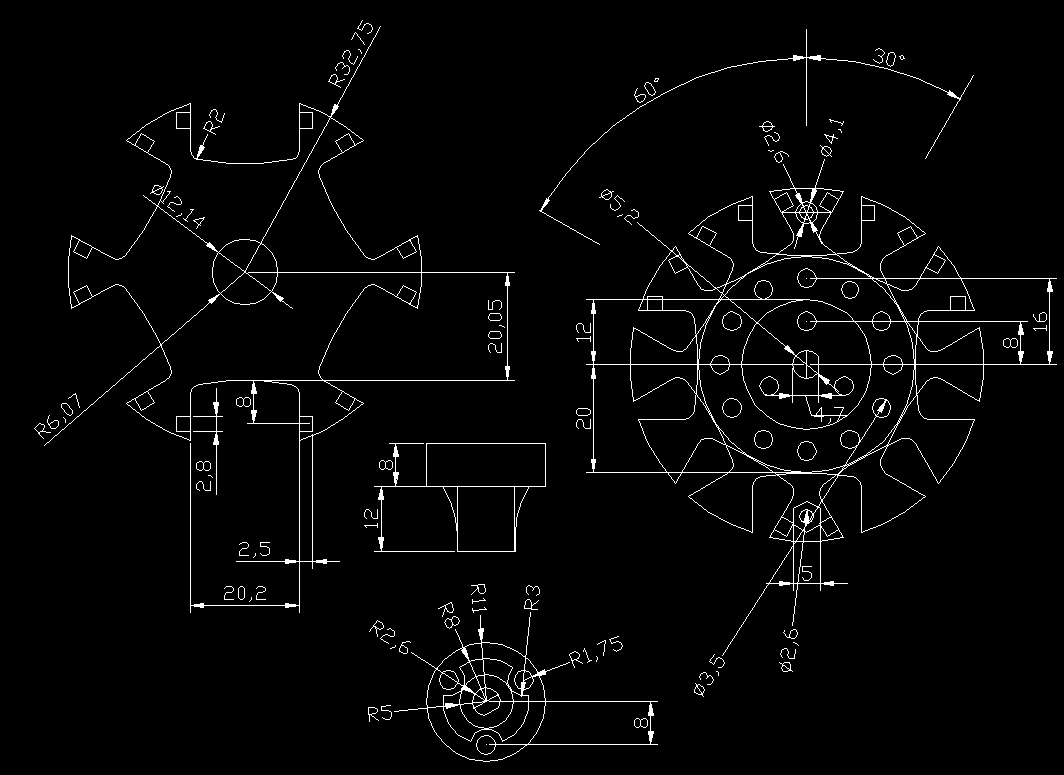
\includegraphics[width=0.9\textwidth]{figures/roda_processo_desing_passo1}
    \caption*{FONTE: Própria}
\end{figure}

\begin{figure}[h]
	\centering
	\caption{Estudo e testes do design da nova roda}
	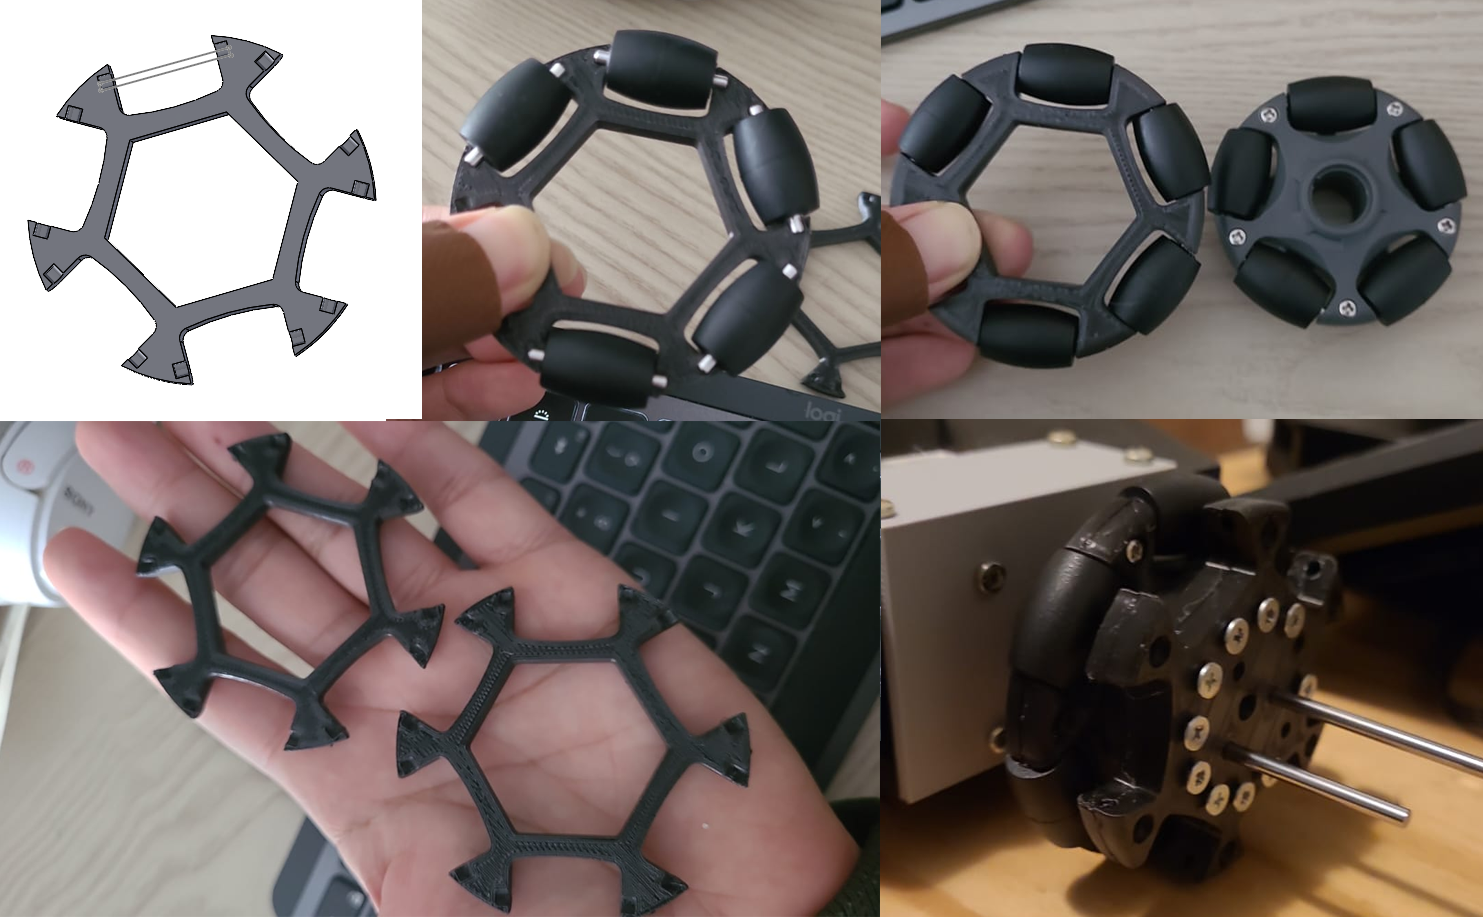
\includegraphics[width=0.9\textwidth]{figures/estudo_roda}
    \caption*{FONTE: Própria}
\end{figure}

\begin{figure}[h]
	\centering
	\caption{Desing final - Solidworks}
	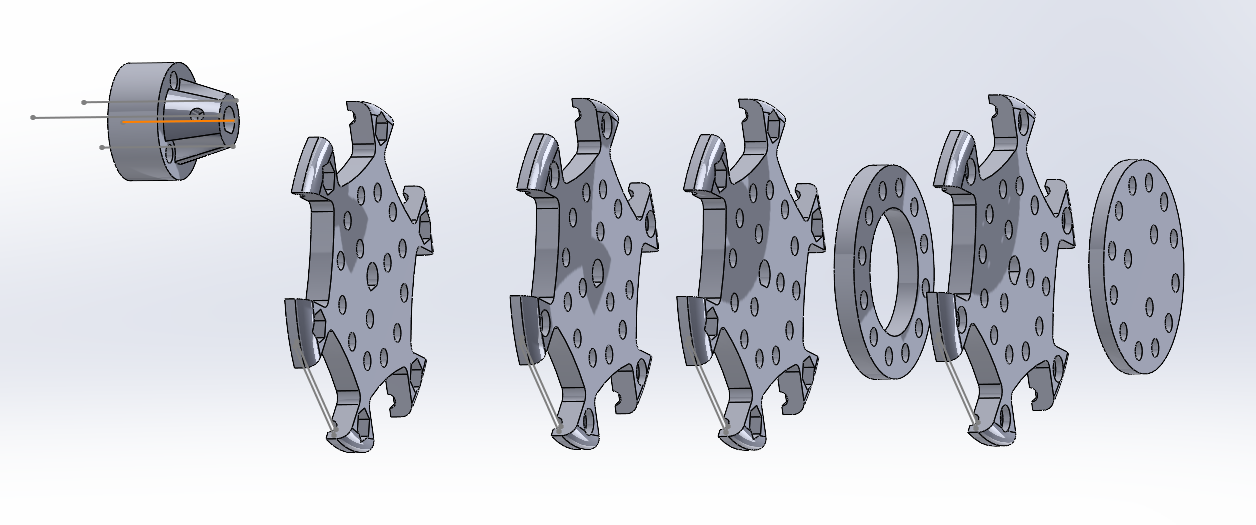
\includegraphics[width=0.9\textwidth]{figures/roda_processo_desing_passo2}
    \caption*{FONTE: Própria}
\end{figure}

\begin{figure}[h]
	\centering
	\caption{Desing final - Preparação para impressão}
	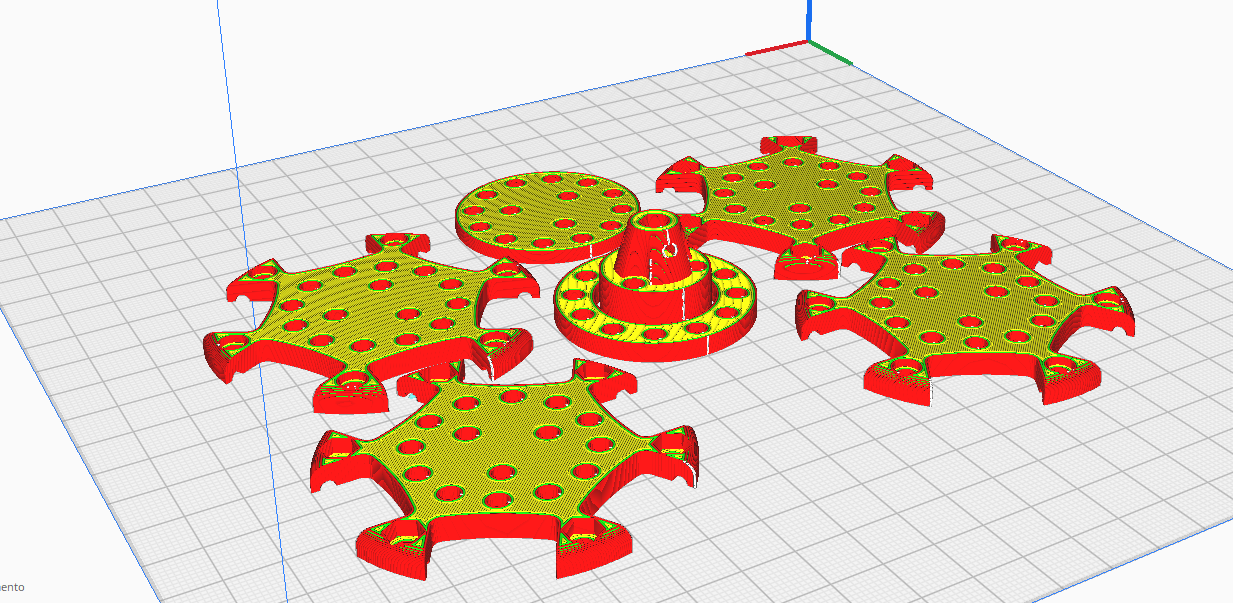
\includegraphics[width=0.9\textwidth]{figures/roda_processo_desing_passo3}
    \caption*{FONTE: Própria}
\end{figure}

\begin{figure}[h]
	\centering
	\caption{Montagem da roda}
	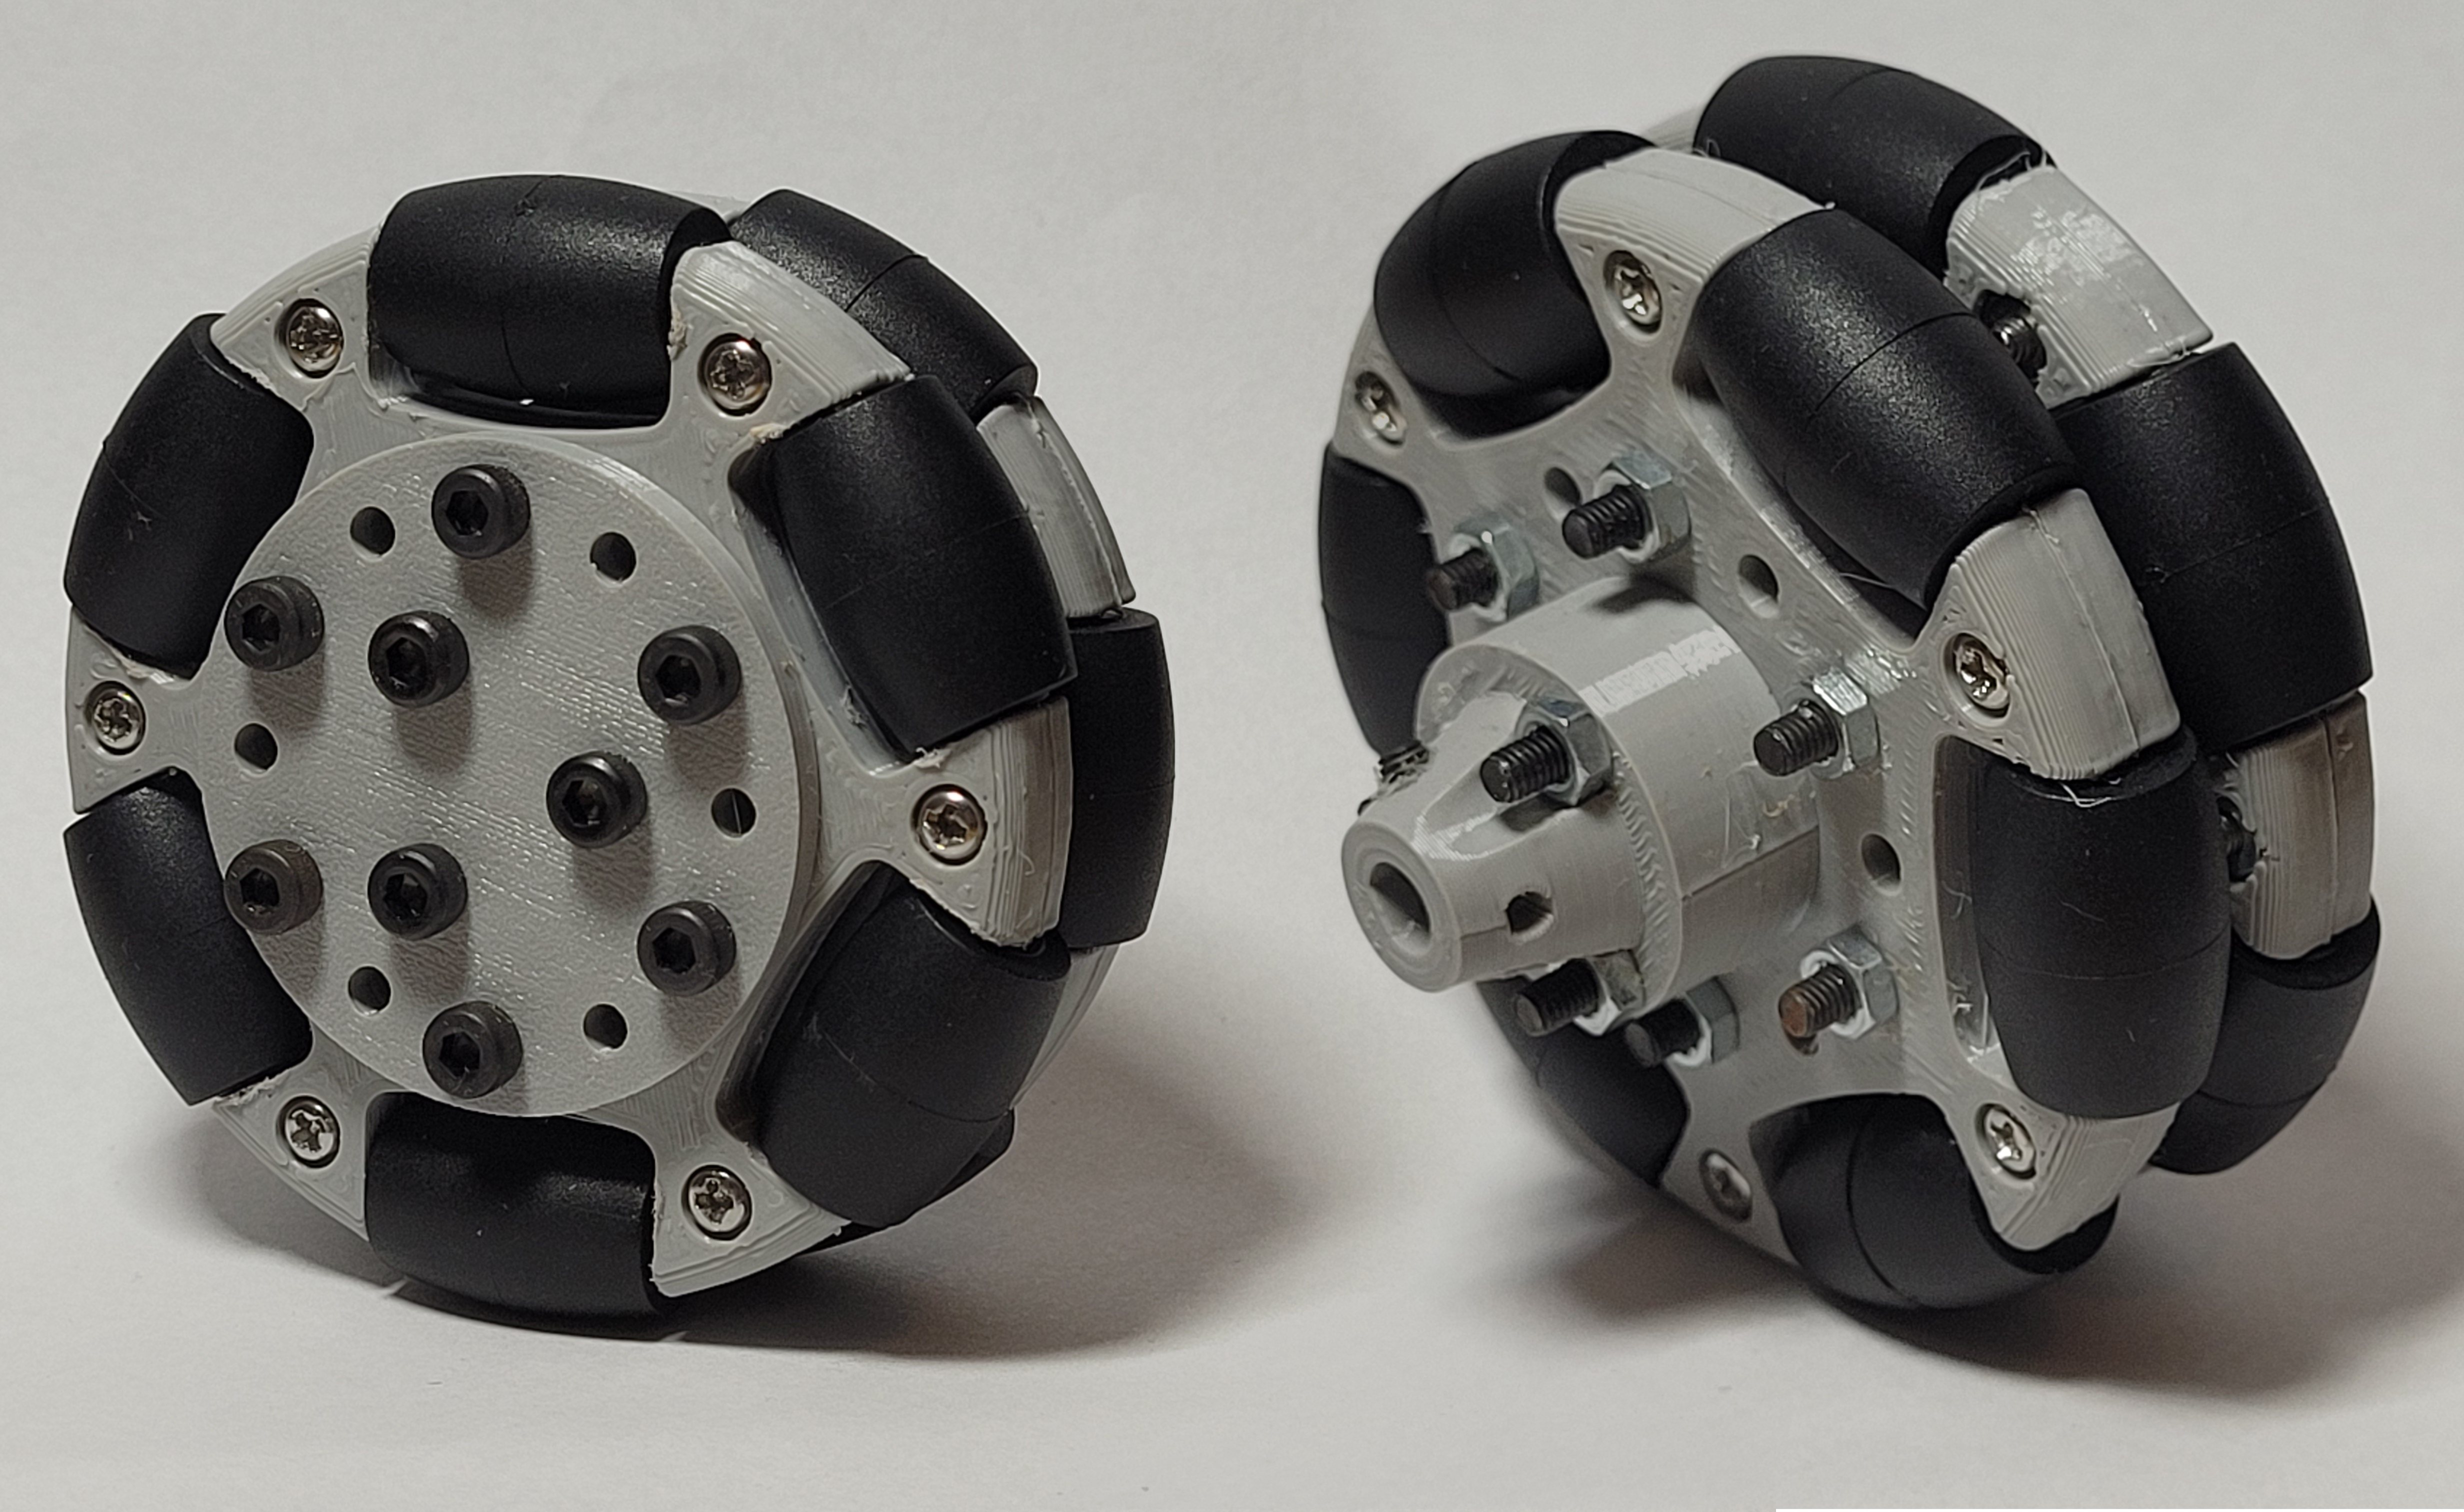
\includegraphics[width=0.9\textwidth]{figures/roda_processo_desing_passo4}
    \caption*{FONTE: Própria}
\end{figure}